\documentclass{beamer}
\usepackage[utf8]{inputenc}
\usetheme{Copenhagen}
\usepackage{graphicx}
\graphicspath{ {/tcp/} }
\usepackage[spanish]{babel}
\selectlanguage{spanish}
\usepackage{array}
\usepackage{enumitem}
%Information to be included in the title page:
\title{TCP (Transmission Control Protocol) \\Protocolos E2E}
\author{Antunez Joaquin, Gonzalez Alejo y Nielsen Maximiliano}
\institute{Instituto Politecnico Superior}
\date{2019}


\begin{document}
	
	\frame{\titlepage}
	
	\begin{frame}
		\frametitle{Modelo OSI}
			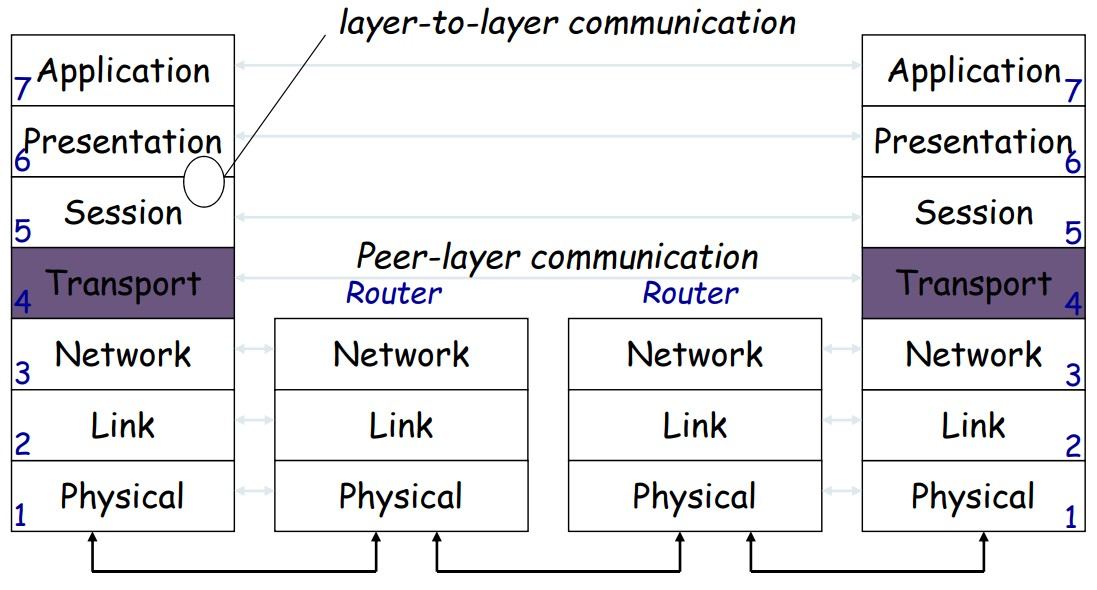
\includegraphics[width=\textwidth]{modeloOSI}
			\begin{center}
				(Fig. 1)
			\end{center}
	\end{frame}


	\begin{frame}
		\frametitle{Modelo OSI}
		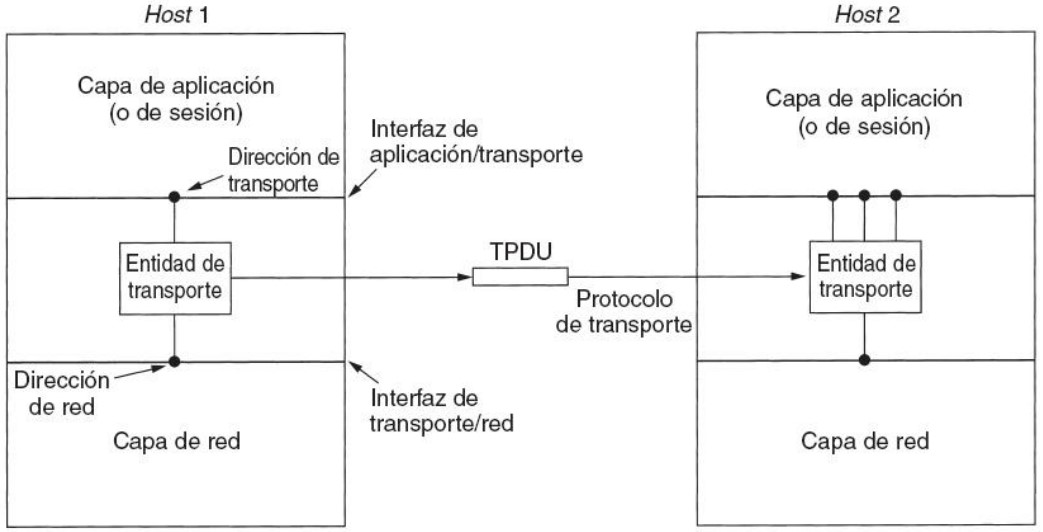
\includegraphics[width=\textwidth]{capas}
		\begin{center}
			(Fig. 2)
		\end{center}
	\end{frame}
	\begin{frame}
		\frametitle{Modelo OSI}
 	En la figura 2 podemos ver como es la comunicación de un TPDU.\\
	El Host emisor cuenta con una interfaz entre la capa de aplicación y la de transporte que le provee de una Dirección de transporte para la aplicación. La entidad de transporte genera la TPDU que luego será transmitida hacia la interfaz de transporte/red para que la capa de red se encargue de la transmisión.\\
 	Una vez que la TPDU arriba al segundo Host, la capa de transporte se encarga de enviar el PDU hacia la dirección de la aplicación que corresponda
	
	\end{frame}

	\begin{frame}
		\frametitle{Modelo OSI}
			\begin{center}
				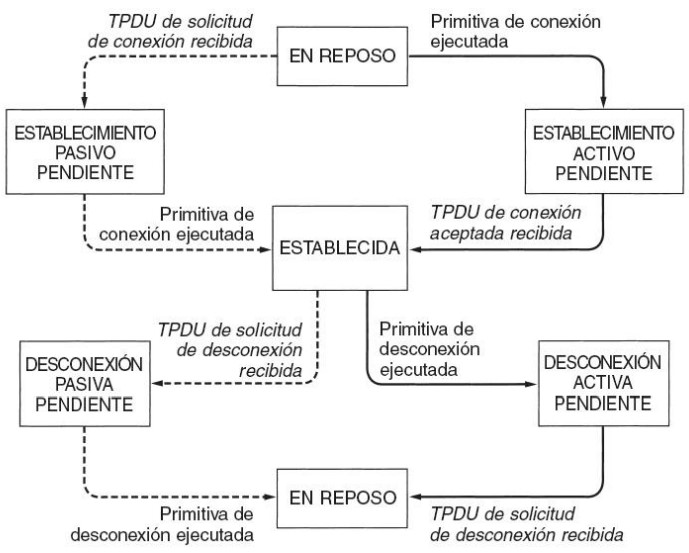
\includegraphics[ scale=0.4]{estados}\\
				{\tiny (Fig. 3)}\\
			{\scriptsize  Diagrama de estados para el manejo de conexiones. Las transiciones escritas en cursivas son causadas por llegadas de paquetes. Las líneas continuas muestran la secuencia de estados del cliente y las líneas punteadas los del servidor.}
			\end{center}
	\end{frame}
	\begin{frame}
		\frametitle{Nivel Transporte : “End to End”}
		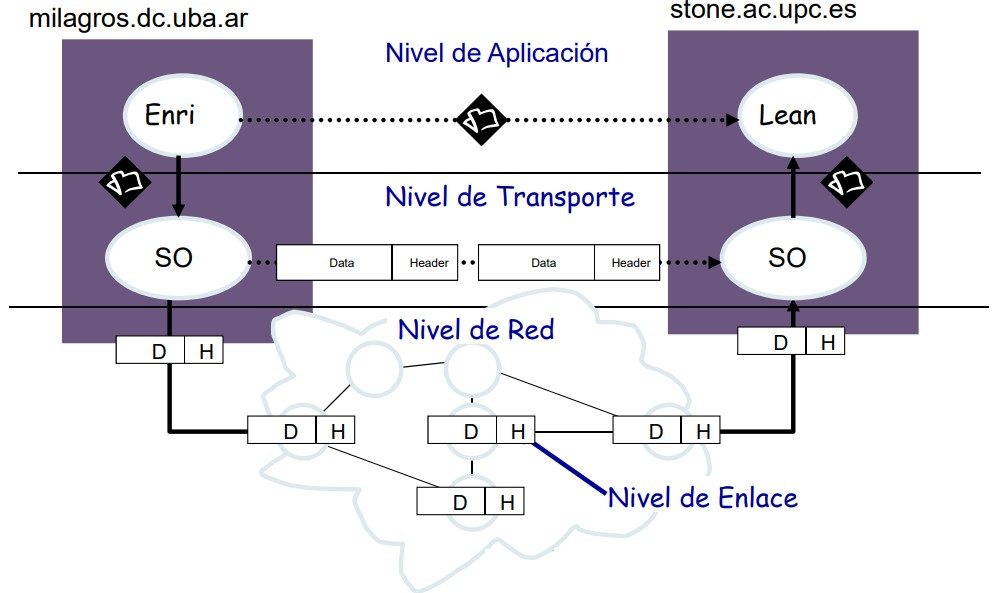
\includegraphics[width=\textwidth]{e2e}
		\begin{center}
		(Fig. 4)
		\end{center}
	\end{frame}
	\begin{frame}
		\frametitle{Enlace de Datos vs Transporte}
	\begin{center}
	
		\begin{tabular}{| m{5cm} | m{5cm}| }
			\hline
			Enlace de Datos & Transporte  \\ 
			 \hline\hline
			 Potencialmente conecta   muchas máquinas diferentes &
			 Requiere de establecimiento y término de conexión explícitos  \\ 
			 \hline 
			Potencialmente diferentes RTT
			&
			Requiere mecanismos adaptivos para timeout \\ 
			\hline
			Potencialmente largos retardos en la red
			&
			Requiere estar preparado par el arribo de paquetes muy antiguos\\
			\hline  
			Potencialmente diferente capacidad en destino
			&
			Requiere acomodar diferentes capacidades de nodos\\
			\hline
			Potencialmente diferente capacidad de red
			&
			Requiere estar preparado para congestión en la red\\
			\hline
		\end{tabular}
	\end{center}
	\end{frame}
	\begin{frame}
	\frametitle{Protocolos E2E en subredes datagramas}
	  \begin{description}
	  	\item[$\bullet$] Si el protocolo E2E se apoya en la capa de Red, la cual al ser best-effort puede producir:\\
	  	\item[$\ast$] mensajes descartados 
	  	\item[$\ast$] mensajes re-ordenados
	  	\item[$\ast$] entregas de múltiples copias de un mensaje dado 
	    \item[$\ast$] mensajes entregados después de un tiempo arbitrariamente largo  
	    \item[$\ast$] limita los mensajes a algún tamaño finito
	  	
	  \end{description}
	  
	\end{frame}
	\begin{frame}
	\frametitle{Protocolos E2E en subredes datagramas}
	\begin{description}
		\item[$\bullet$] Servicios comunes ofrecidos/deseados end-to-end:
		\item[$\ast$] garantía de entrega de mensajes
		\item[$\ast$] entrega de mensajes en el mismo orden que son enviados
		\item[$\ast$] entrega de a lo sumo una copia de cada mensaje
		\item[$\ast$] soporte para mensajes arbitrariamente largos mensajes  
		\item[$\ast$] soporte de sincronización
		\item[$\ast$] permitir al receptor controlar el flujo de datos del transmisor
		\item[$\ast$]soportar múltiples procesos de nivel aplicación en cada
		máquina
	\end{description}
\end{frame}
\begin{frame}
	\frametitle{Caracteristicas del TCP}
	\begin{description}
		\item[$\bullet$] Orientado a conexión: se debe establecer una conexión antes de transferir datos.
		\item[$\bullet$]Flujo de bytes:
		\quad \item[$\ast$] La app escribe bytes
		\quad \item[$\ast$] TCP envía segmentos
		\quad \item[$\ast$] La app receptora lee bytes
		\item[$\bullet$] Full duplex: dos flujos de bytes, el envio de informacion es posible desde ambos extremos al mismo tiempo.
		\item[$\bullet$]Control de flujo: evita que el Tx
		inunde al receptor
		\item[$\bullet$]Control de congestión: evita que
		el Tx sobrecargue la red
	\end{description}
\end{frame}
\begin{frame}
	\frametitle{Comunicación TCP}
			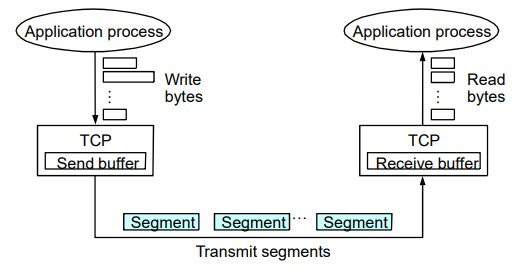
\includegraphics[width=\textwidth]{tcp}
\end{frame}
\begin{frame}


	\frametitle{MSS:”Maximum Segment Size”}
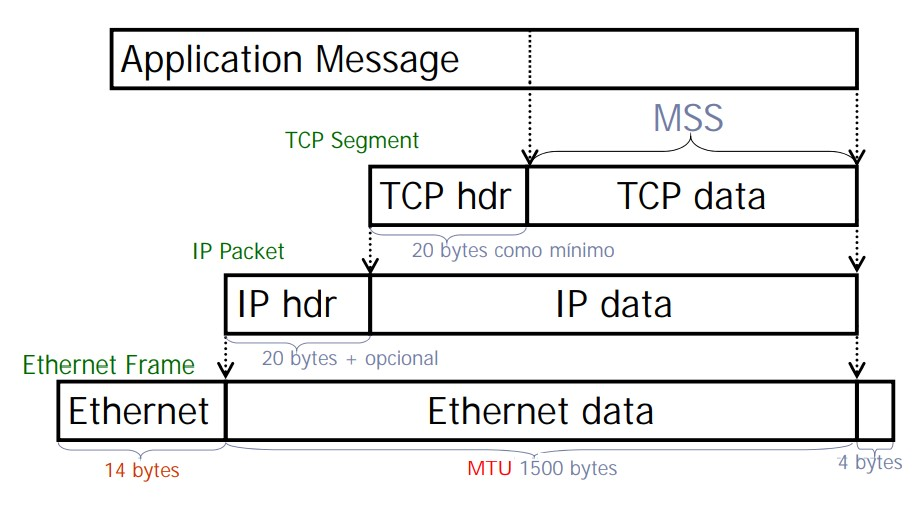
\includegraphics[width=\textwidth]{MSS}
\end{frame}
\end{document}